% Created 2022-10-07 Fri 05:23
% Intended LaTeX compiler: pdflatex
\documentclass[12pt]{article}
\usepackage[utf8]{inputenc}
\usepackage[T1]{fontenc}
\usepackage{graphicx}
\usepackage{longtable}
\usepackage{wrapfig}
\usepackage{rotating}
\usepackage[normalem]{ulem}
\usepackage{amsmath}
\usepackage{amssymb}
\usepackage{capt-of}
\usepackage{hyperref}
\usepackage{fourier}
\usepackage{placeins}
\author{Author list TODO}
\date{}
\title{Appendix title TODO}
\hypersetup{
 pdfauthor={Author list TODO},
 pdftitle={Appendix title TODO},
 pdfkeywords={},
 pdfsubject={},
 pdfcreator={Emacs 28.2 (Org mode 9.5.5)}, 
 pdflang={English}}
\begin{document}

\maketitle
\tableofcontents

\listoffigures


\section{Preamble}
\label{sec:orga0b5156}

TODO

\begin{figure}
\centering
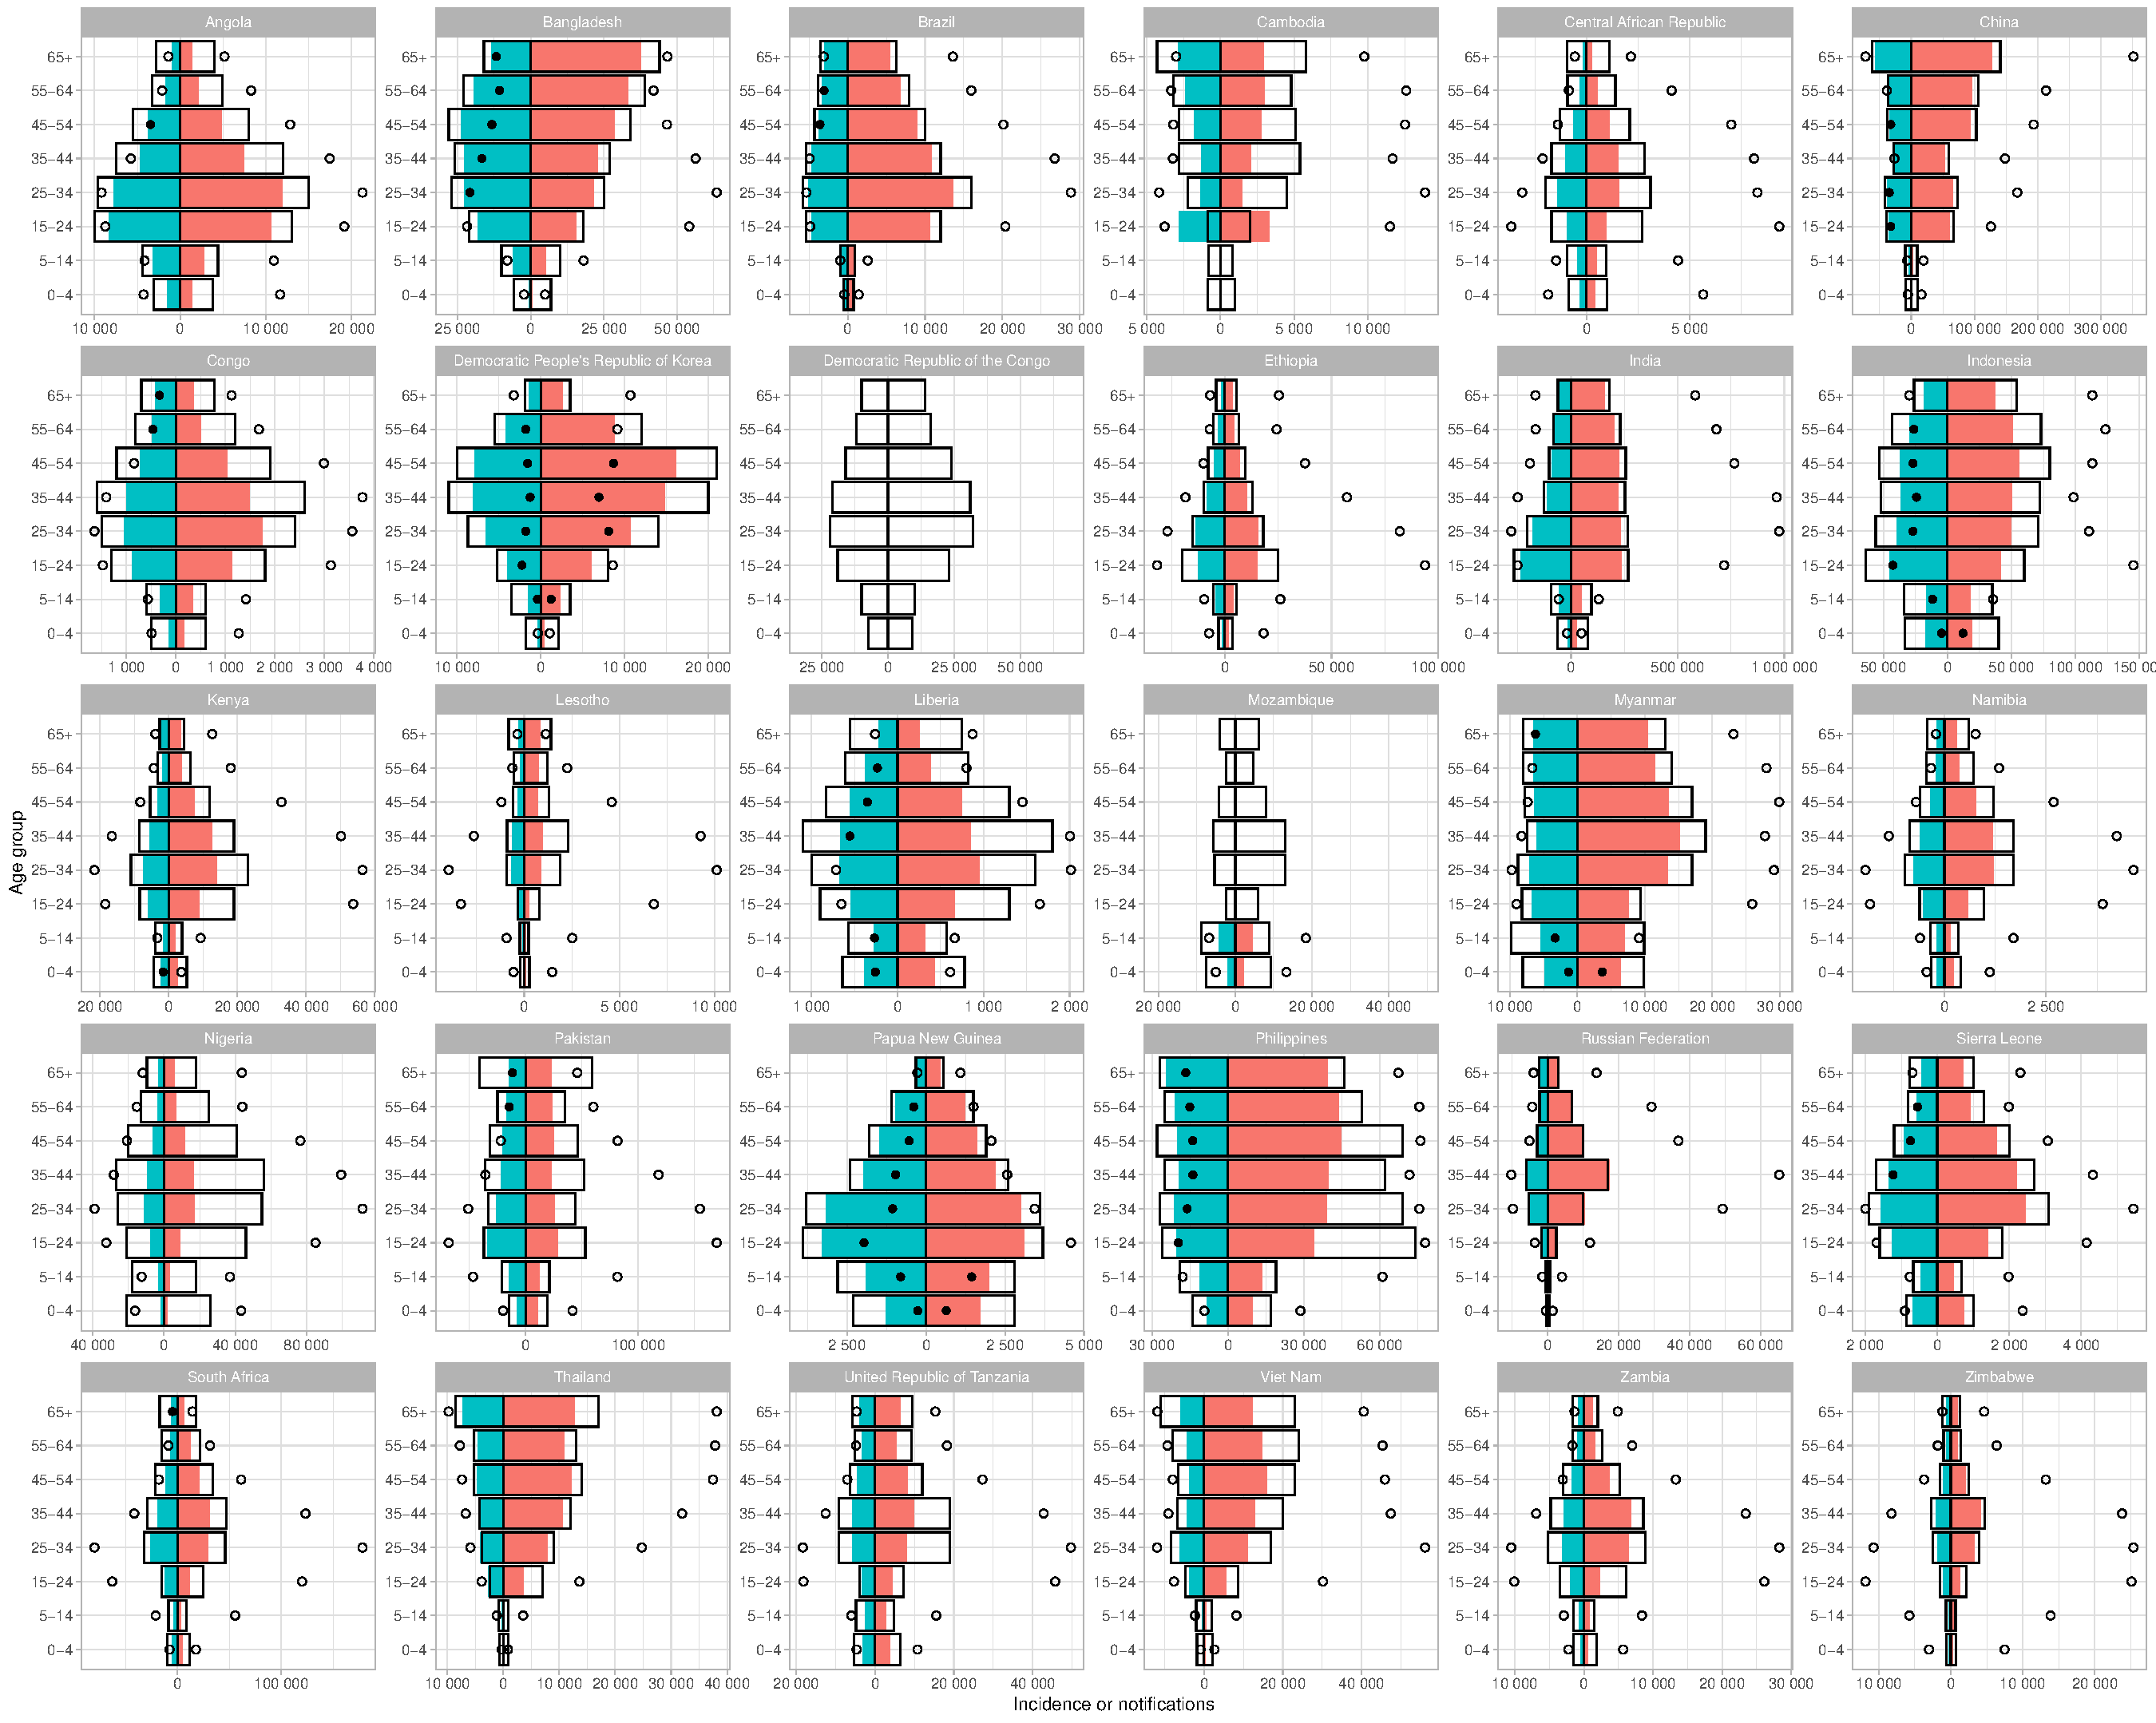
\includegraphics[width=1\textwidth]{../plots/aF1.pdf}
\caption{30 HBC incidence and notifications}
\end{figure}


\FloatBarrier


\begin{figure}
\centering
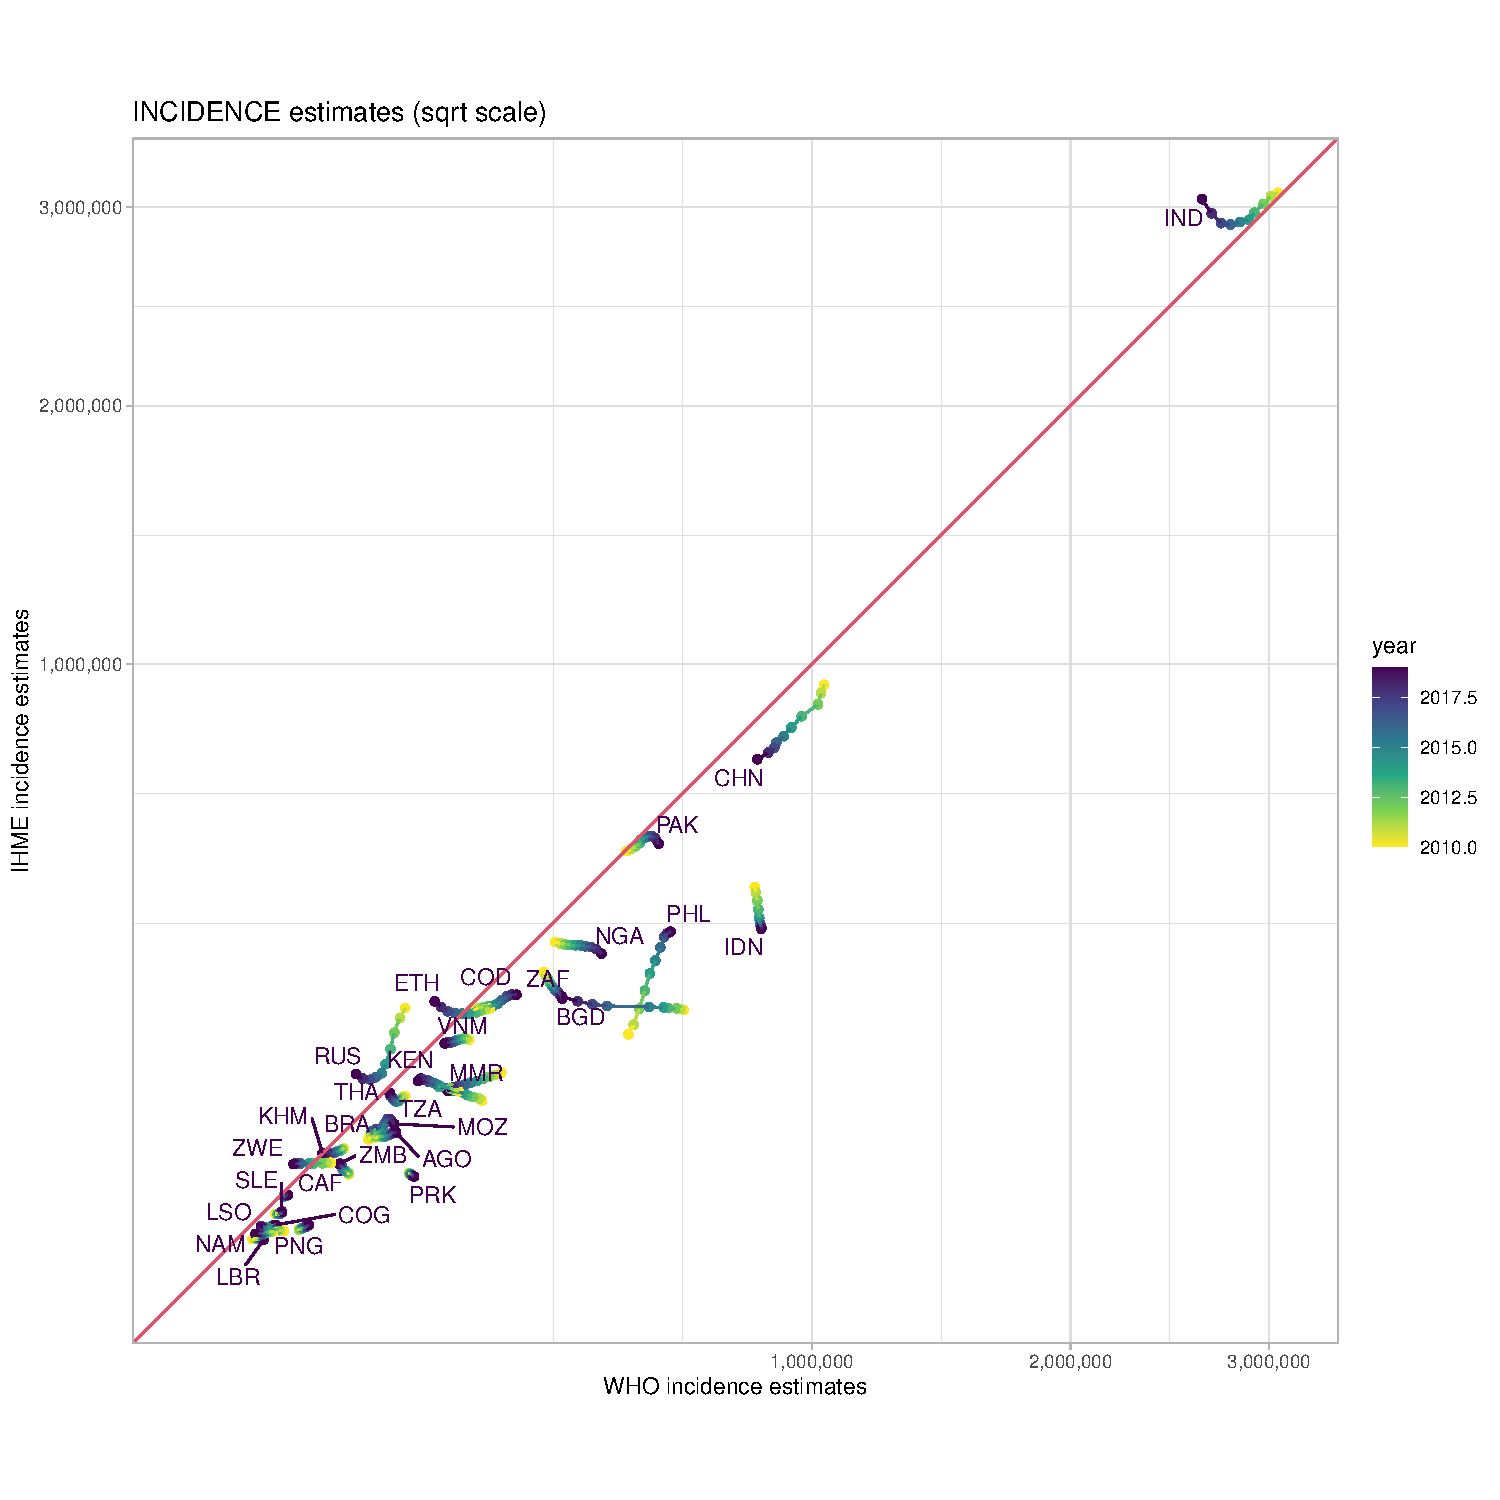
\includegraphics[width=1\textwidth]{../plots/aF2a.pdf}
\caption{Incidence comparison over time}
\end{figure}


\FloatBarrier

\begin{figure}
\centering
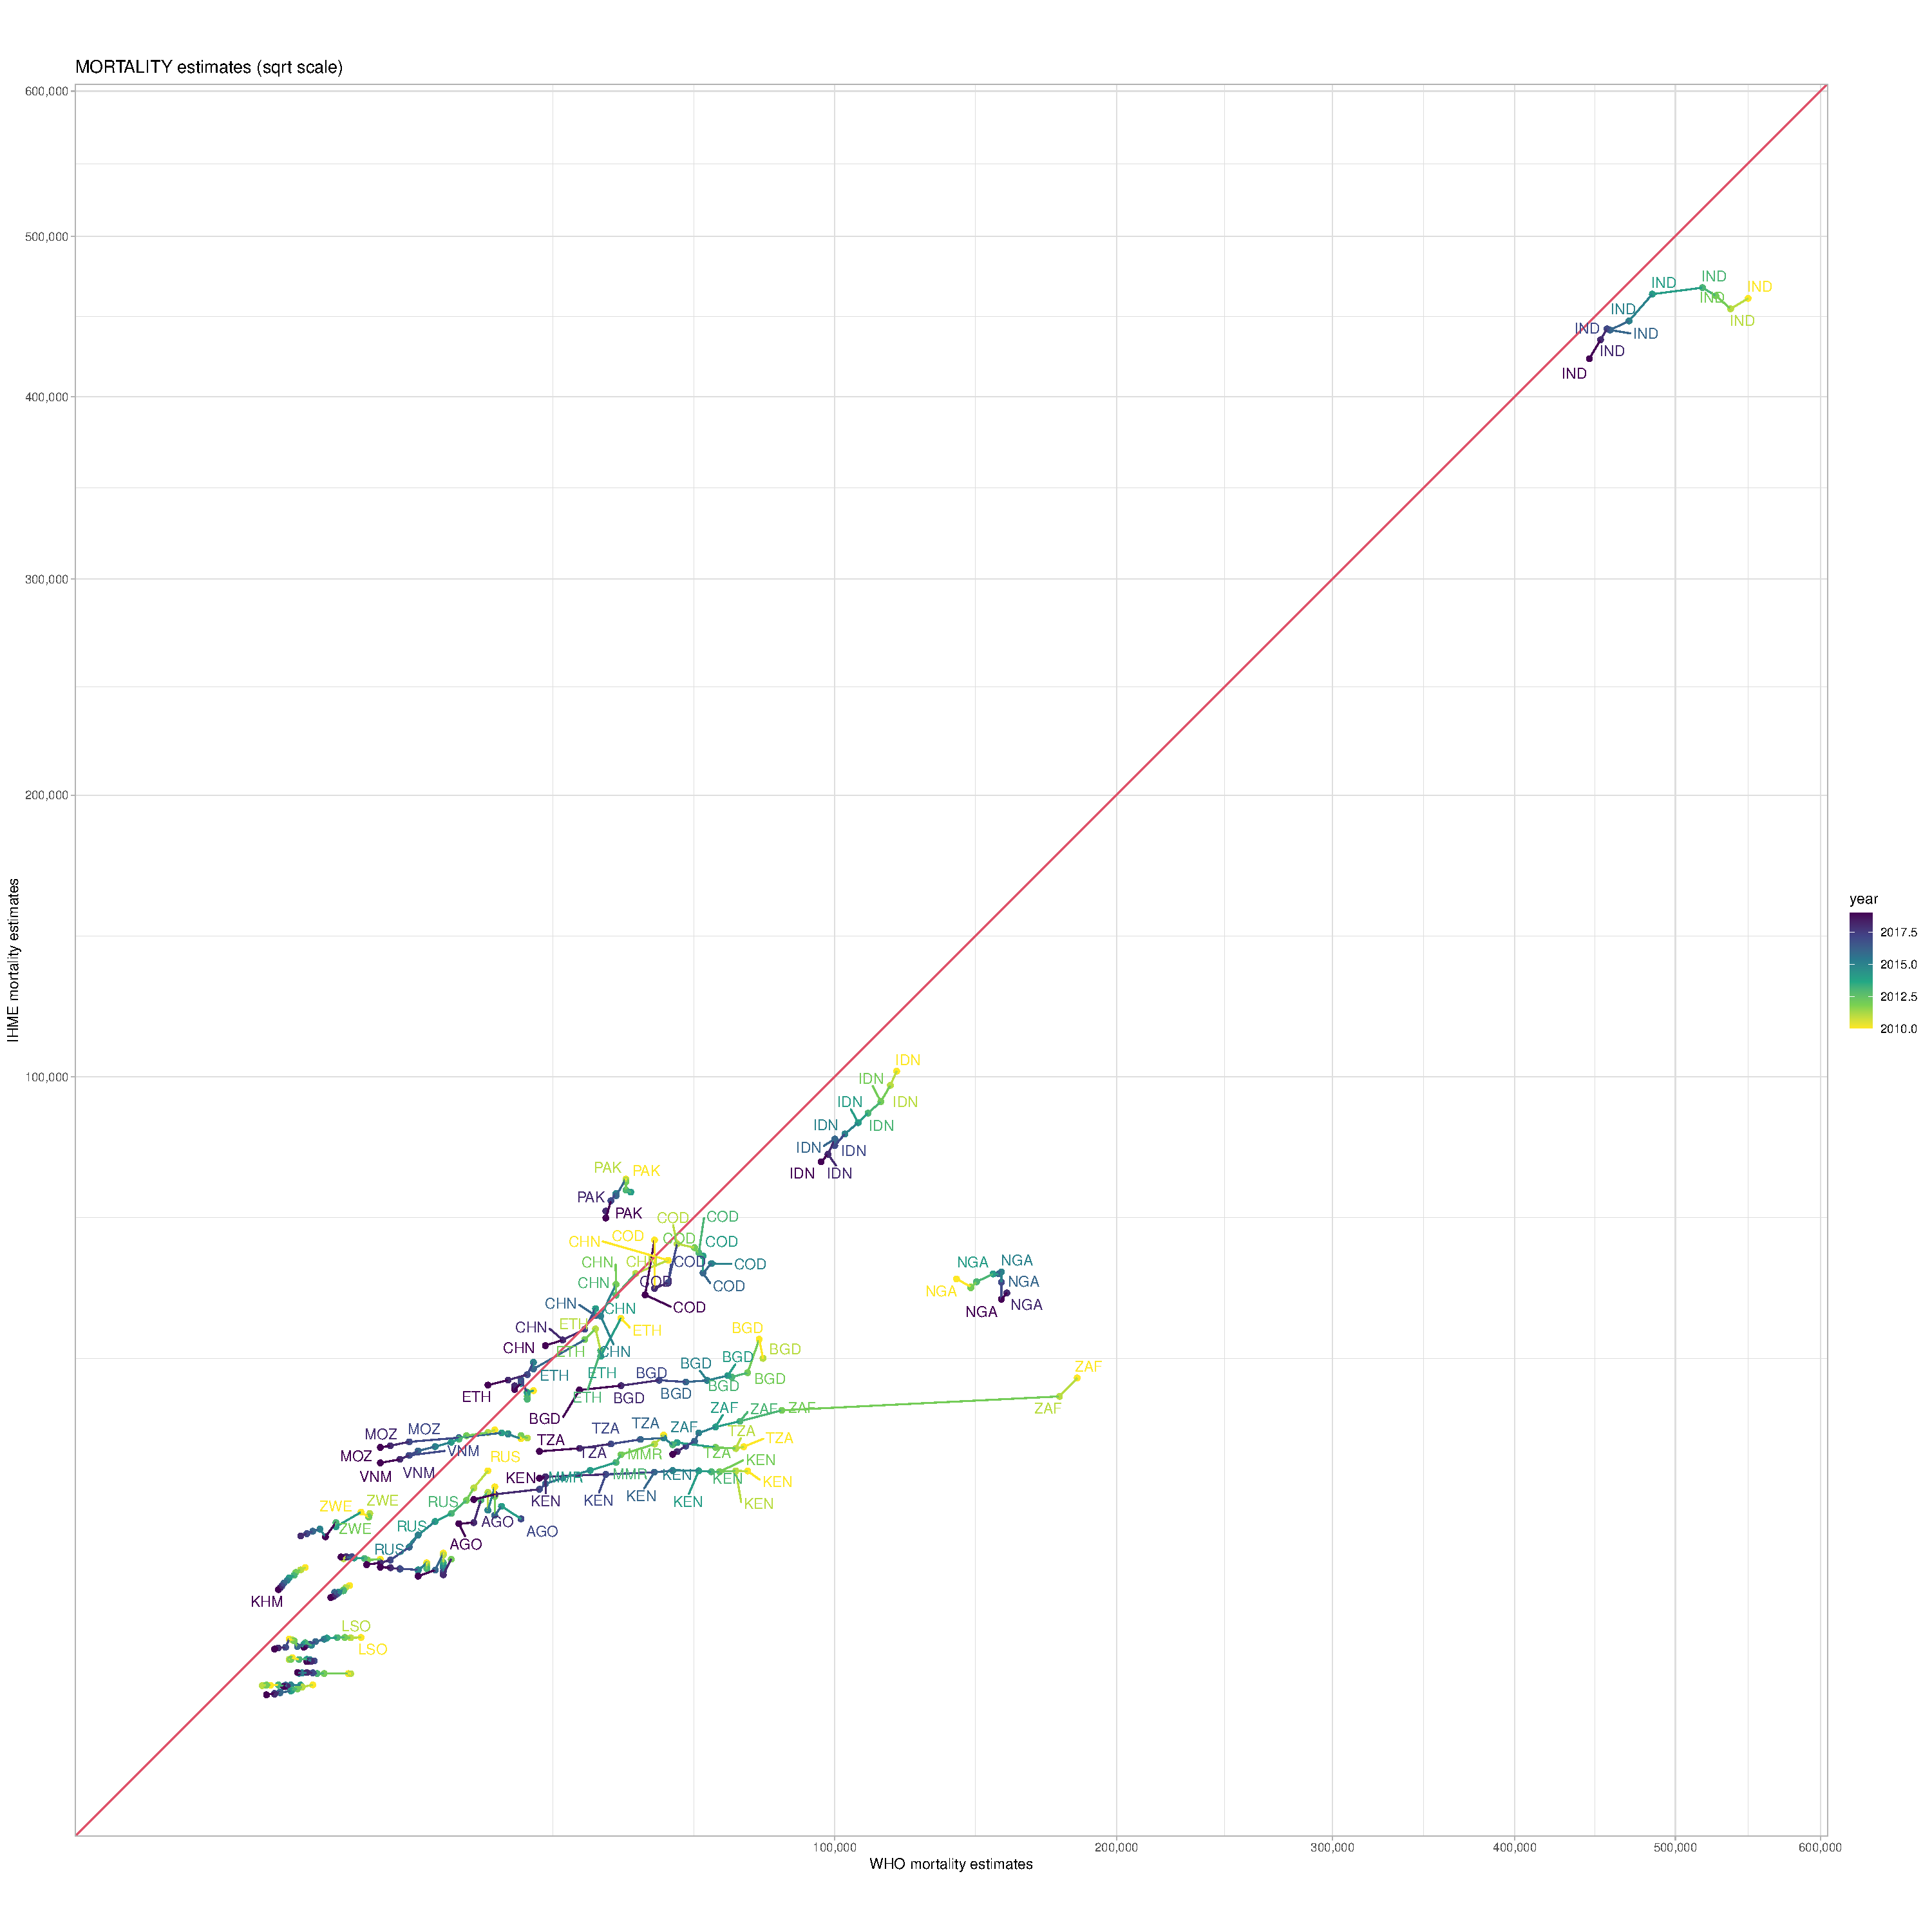
\includegraphics[width=1\textwidth]{../plots/aF2b.pdf}
\caption{Mortality comparison over time}
\end{figure}

\FloatBarrier

\begin{figure}
\centering
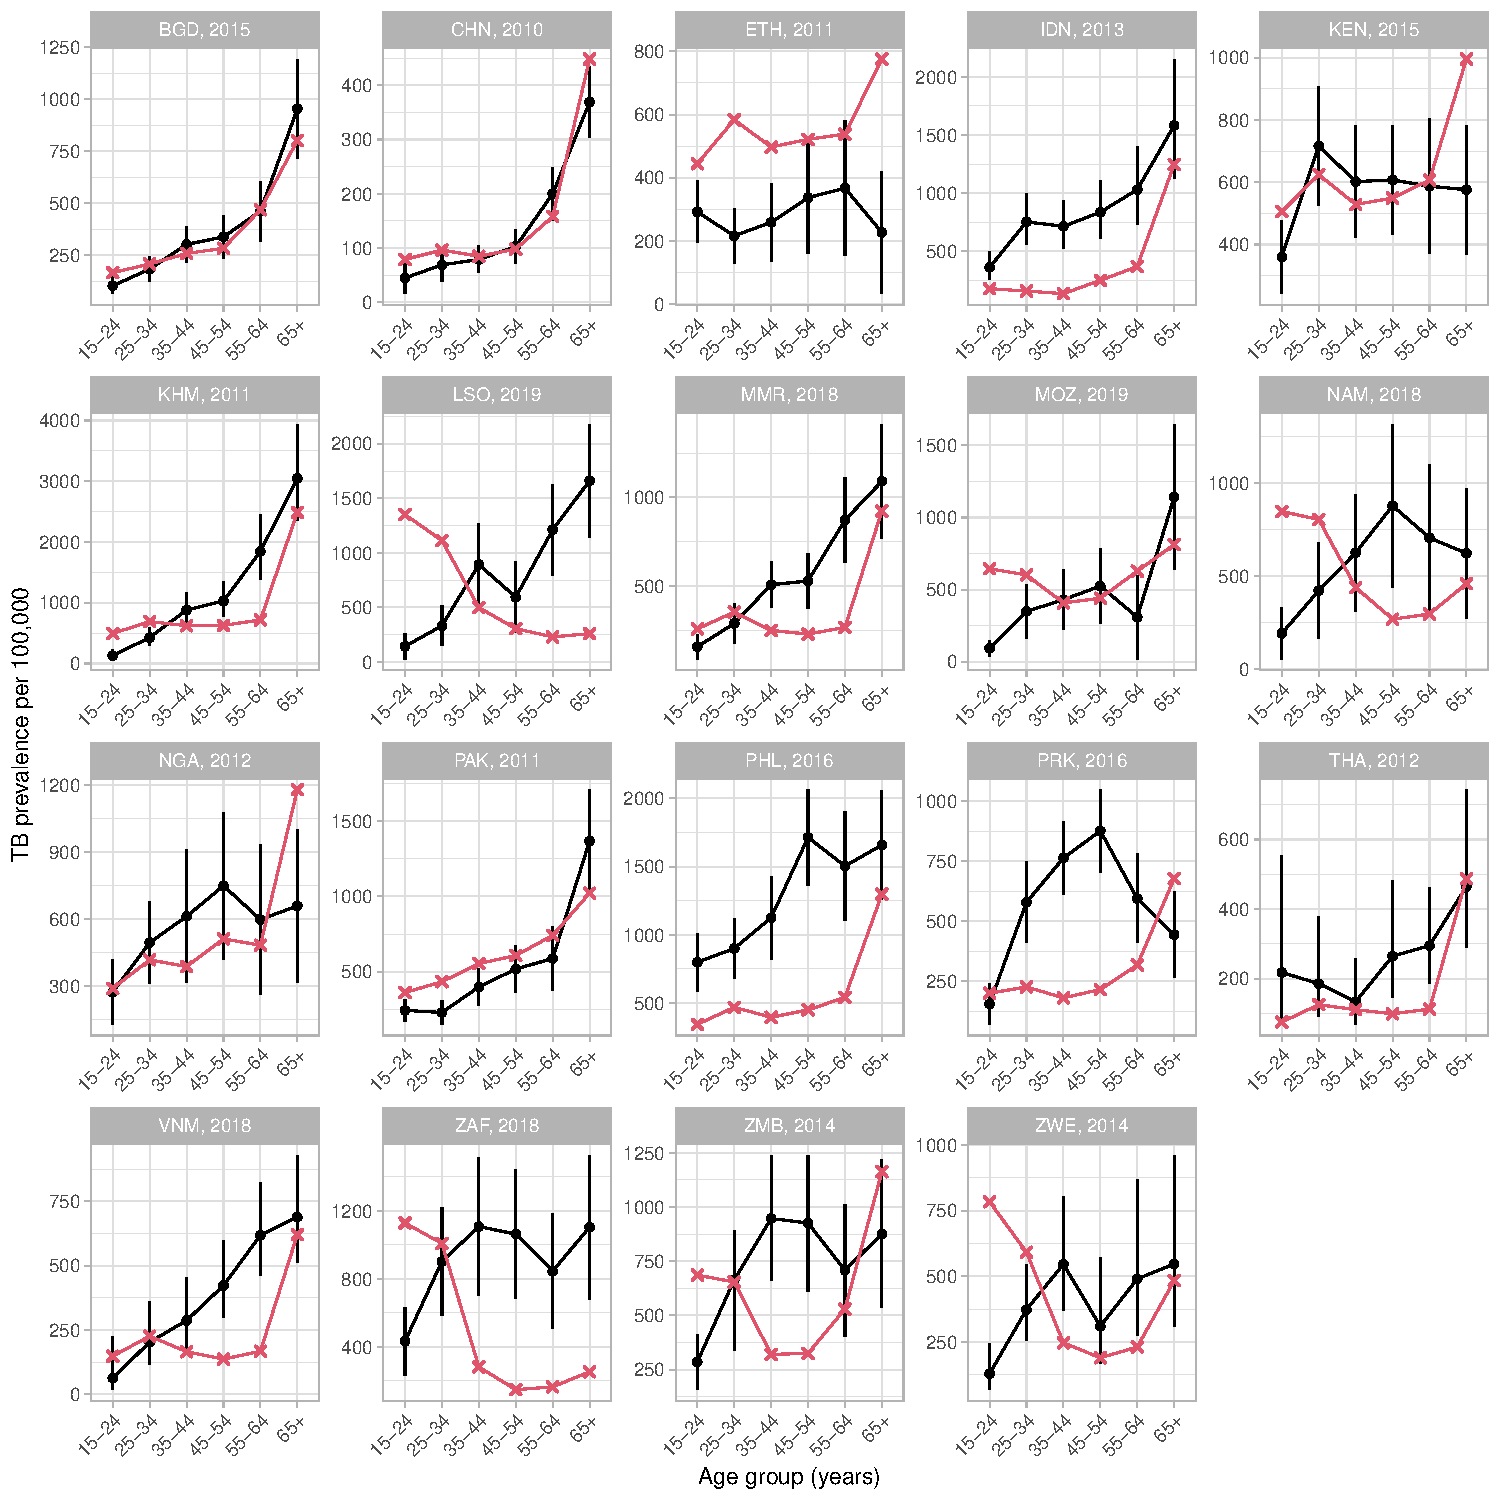
\includegraphics[width=1\textwidth]{../plots/aF3.pdf}
\caption{Prevalence vs prevalence survey. Red=IHME all TB prevalence point
  estimate; black=prevalence survey bacteriologically-confirmed TB prevalence
  and 95\% confidence interval}
\end{figure}


\FloatBarrier

\begin{figure}
\centering
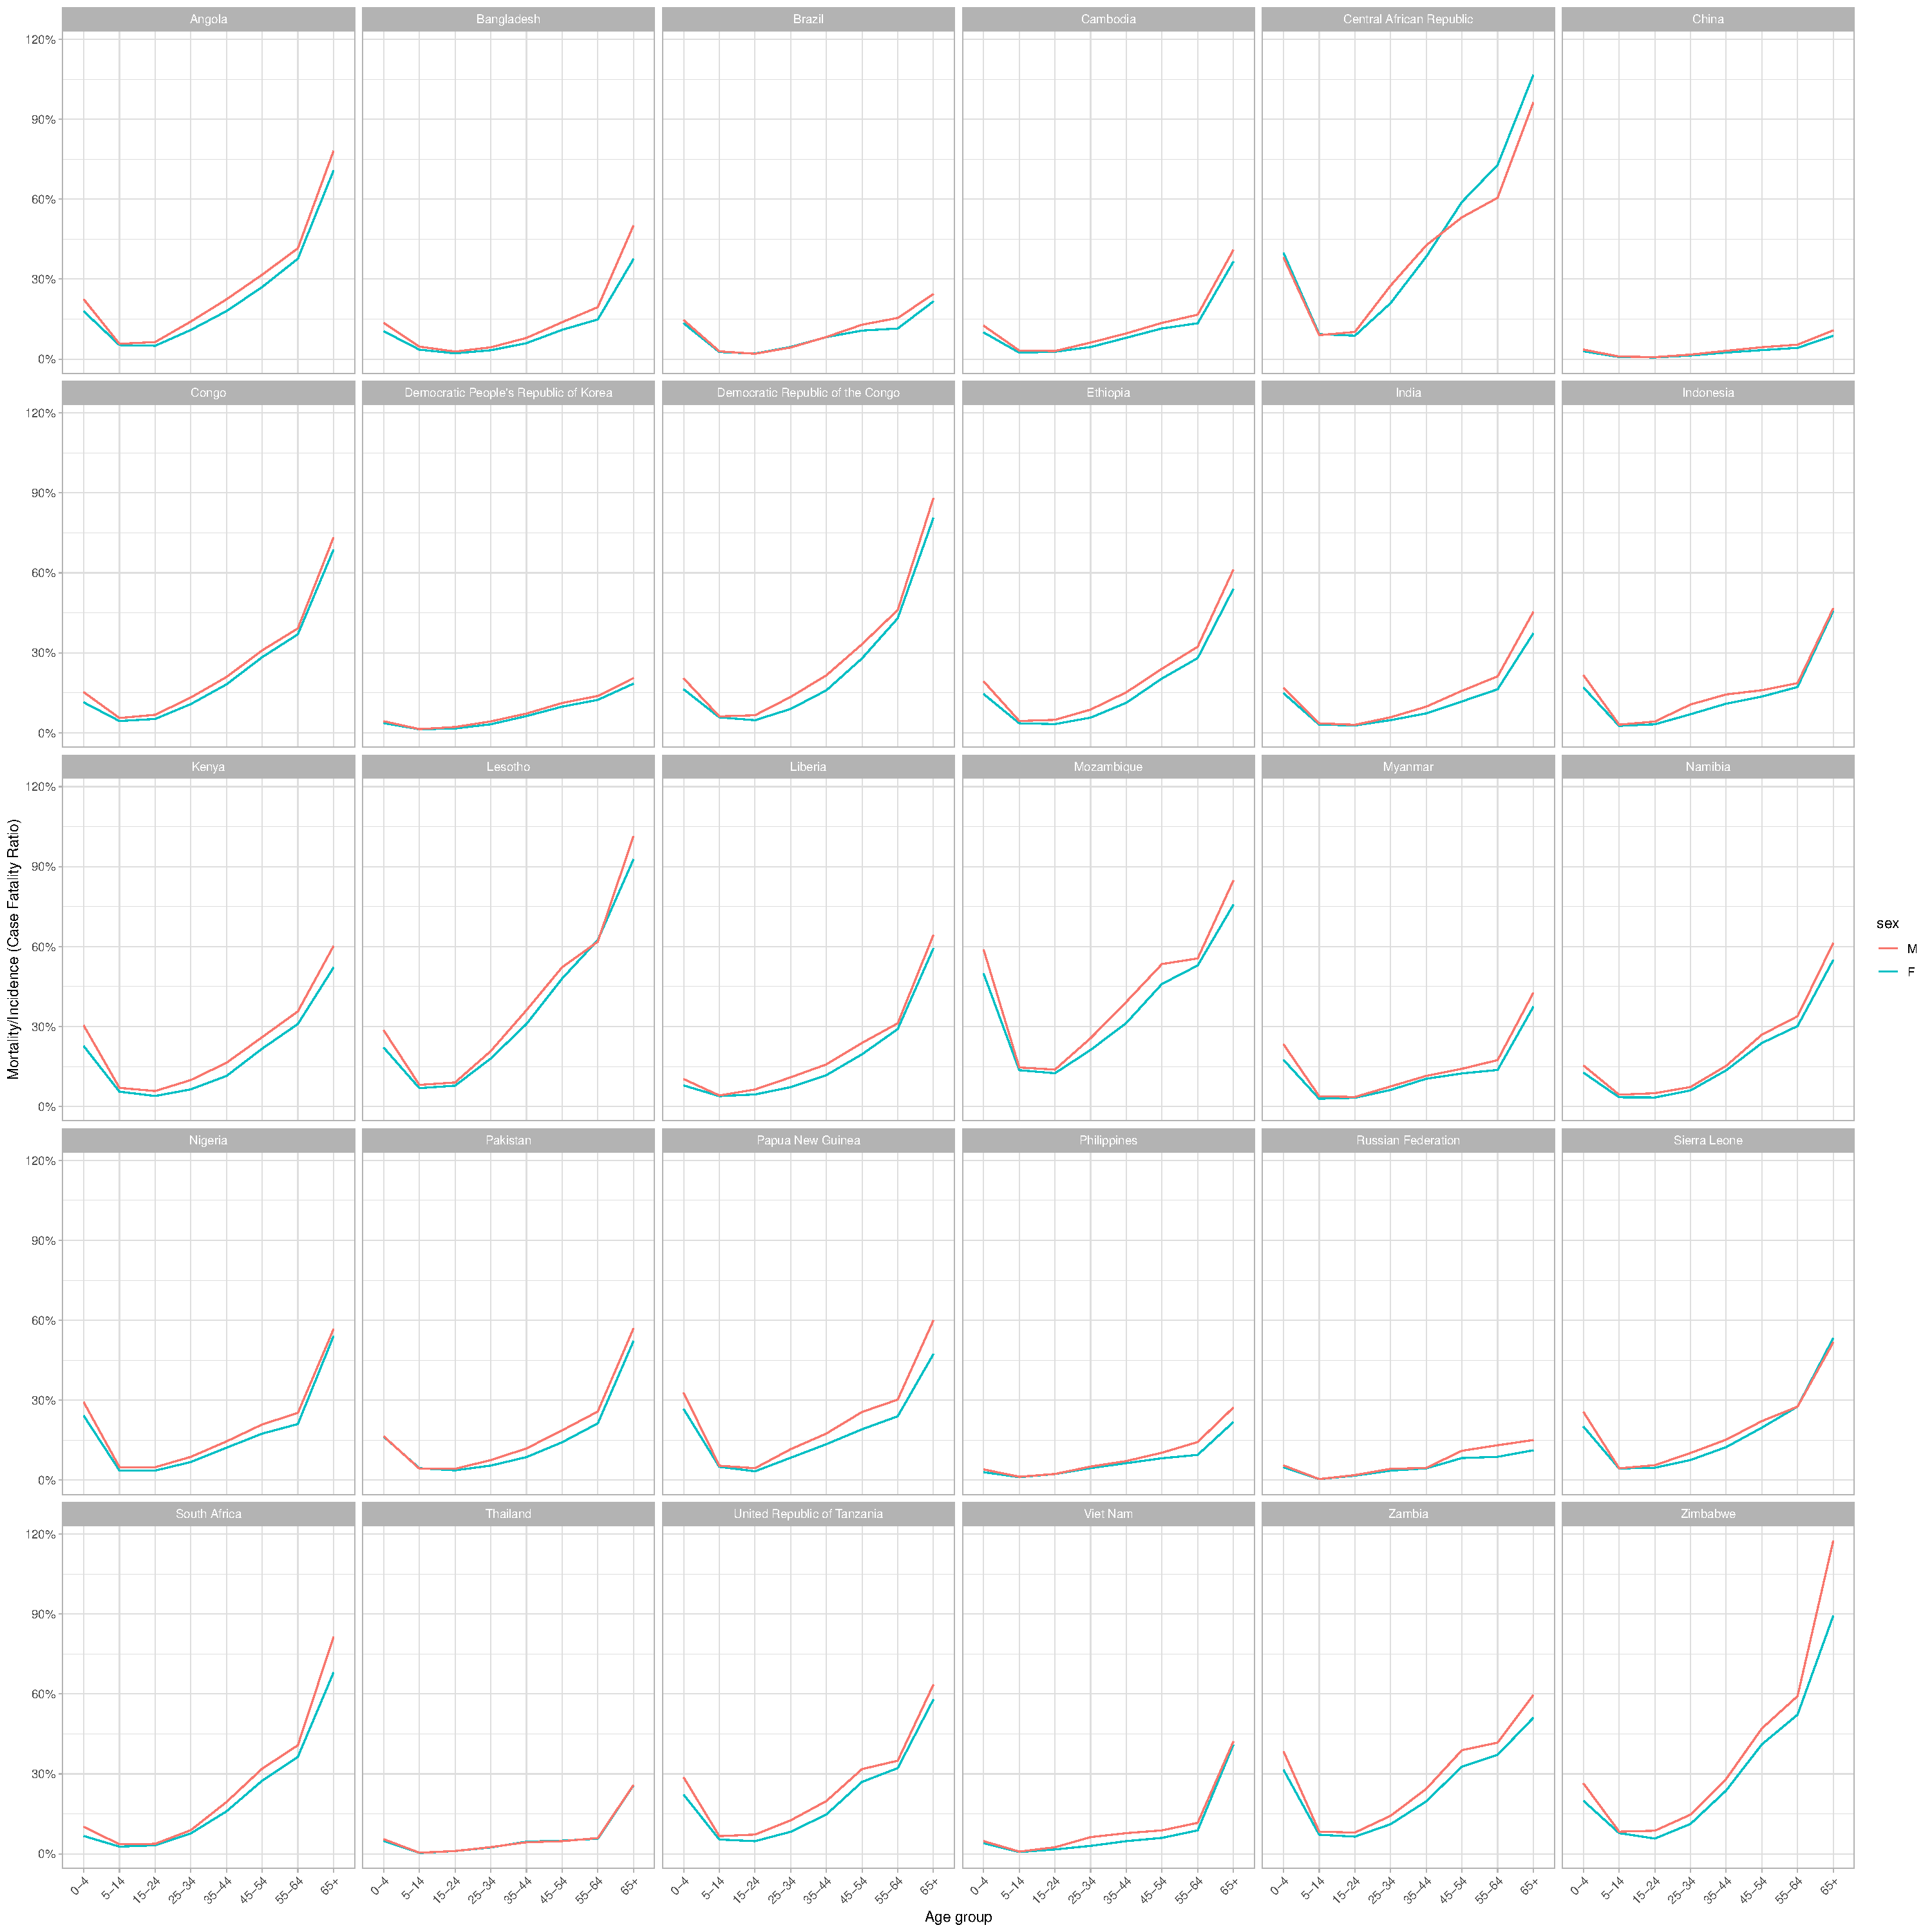
\includegraphics[width=1\textwidth]{../plots/aF4.pdf}
\caption{Case Fatality Ratio by age and sex}
\end{figure}


\FloatBarrier

\begin{figure}
\centering
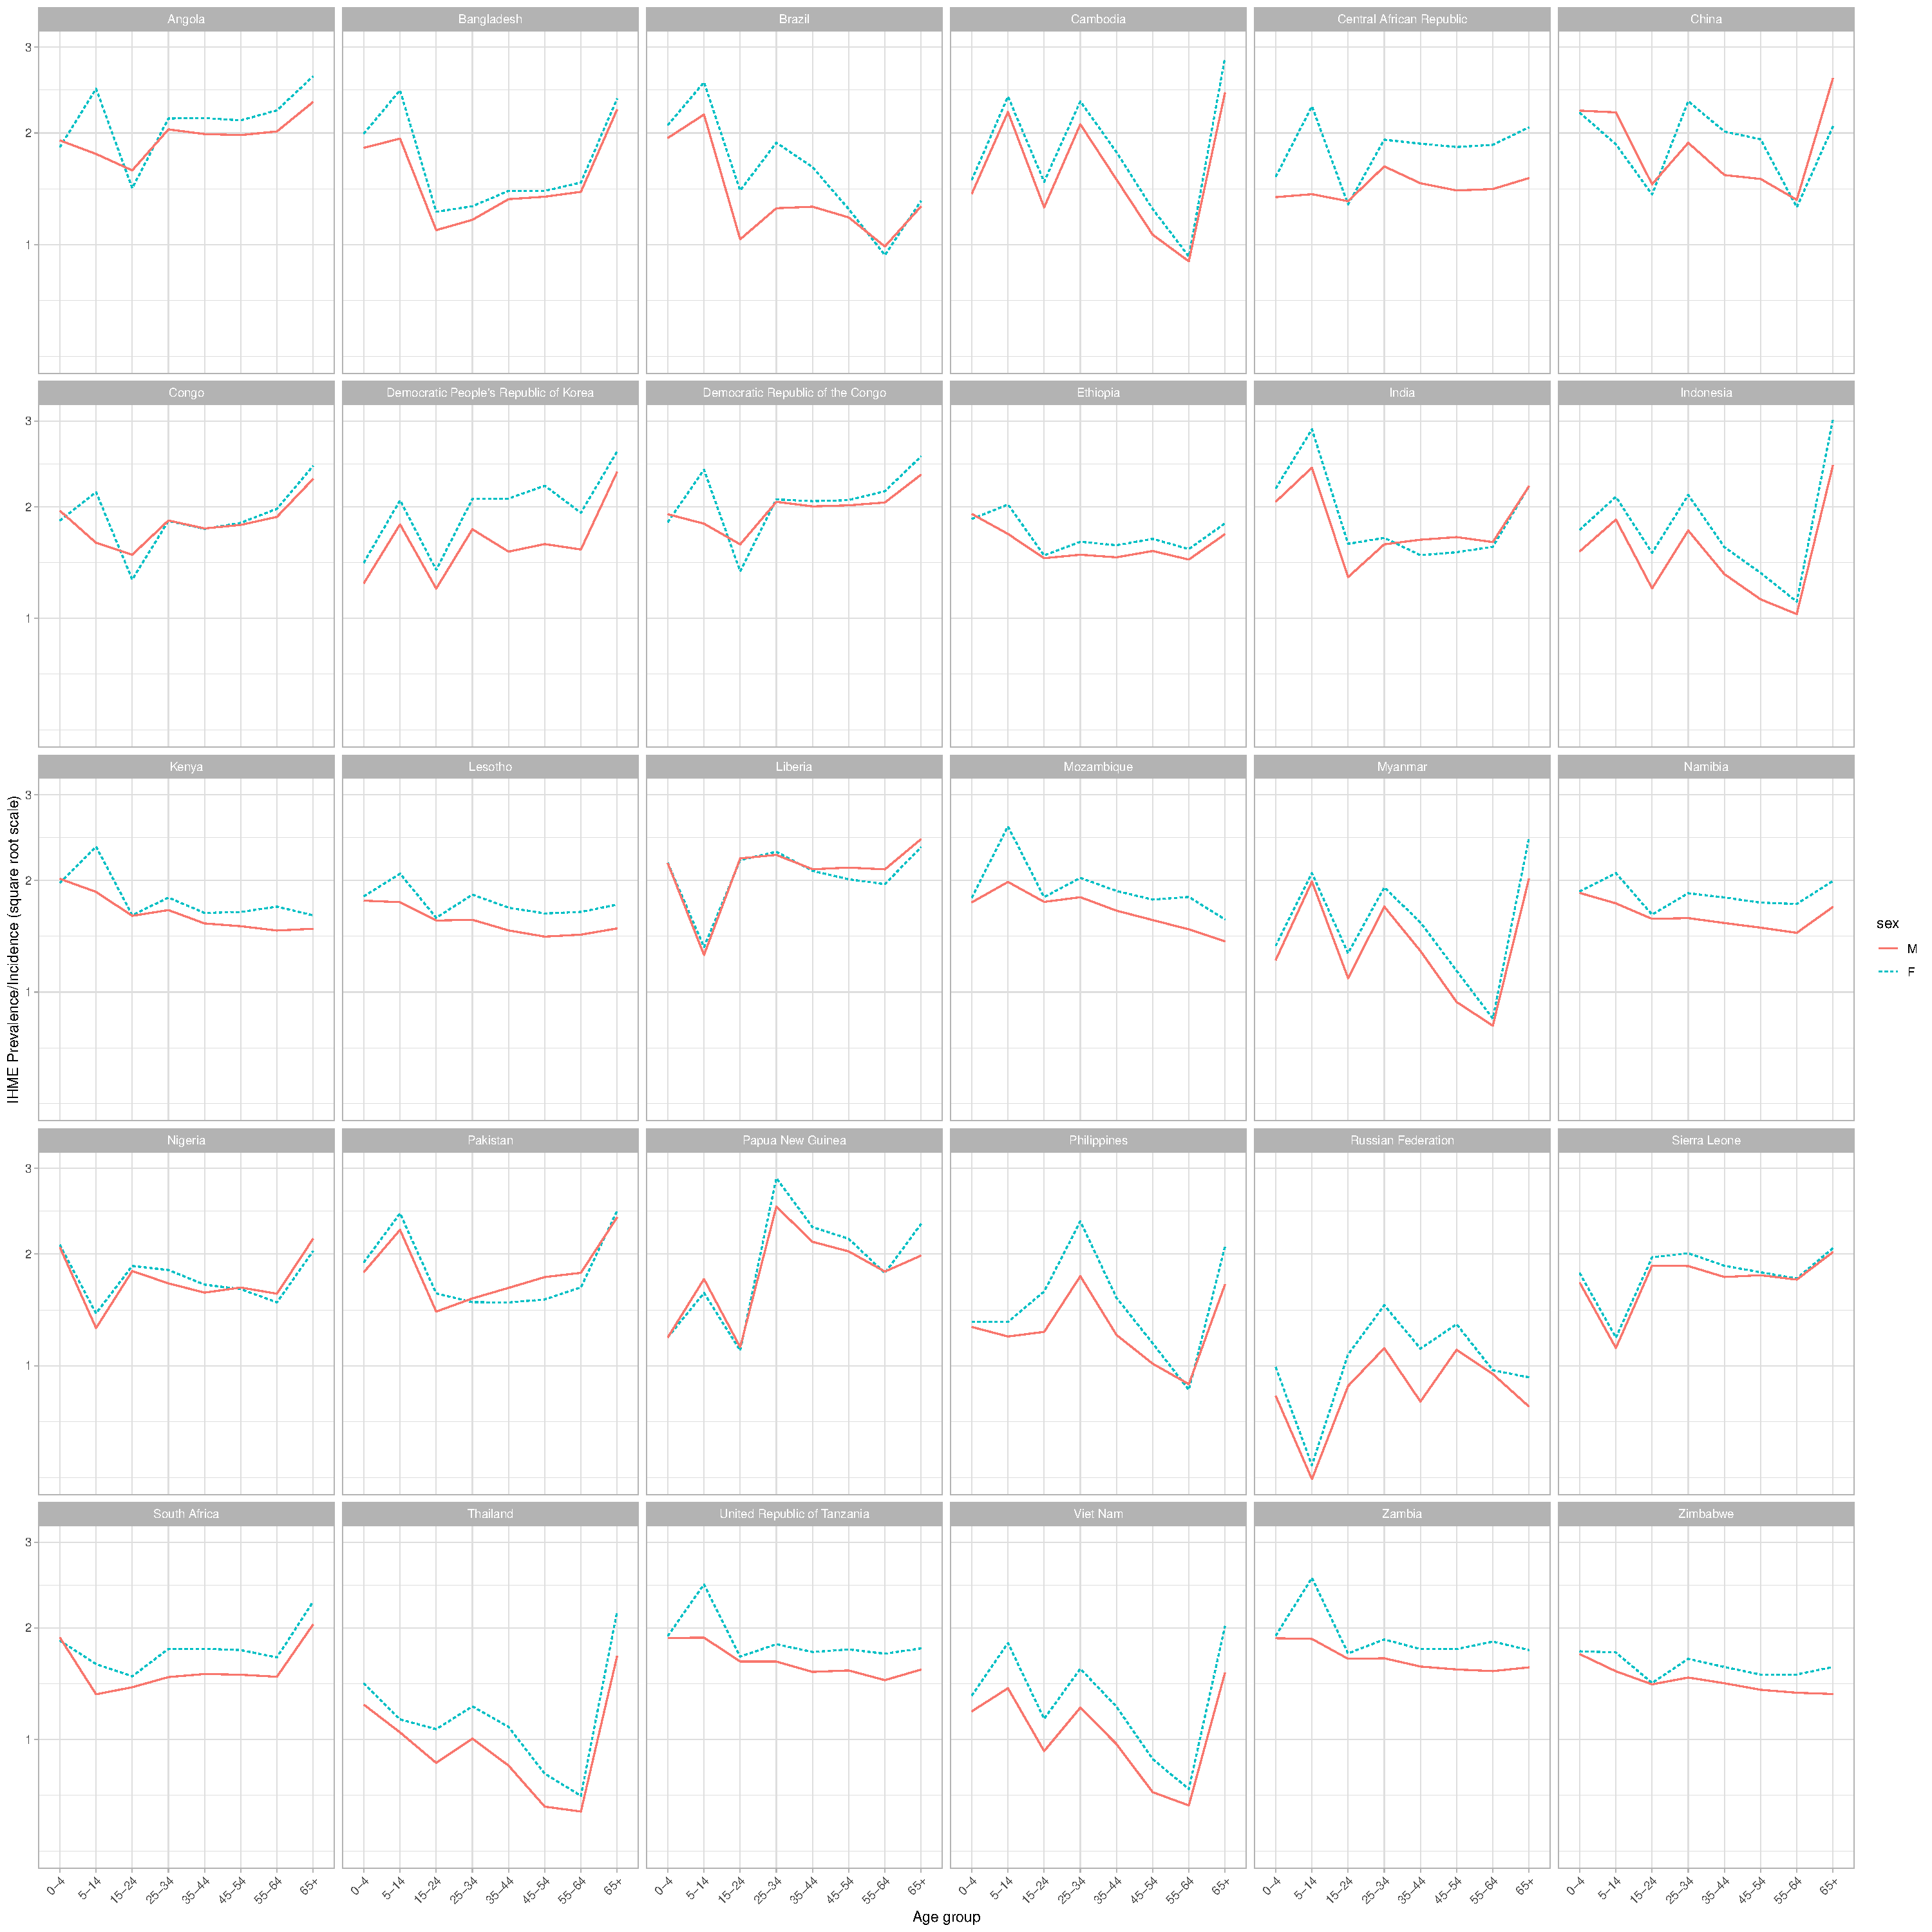
\includegraphics[width=1\textwidth]{../plots/aF5.pdf}
\caption{Implied duration by age and sex}
\end{figure}

\FloatBarrier

\begin{figure}
\centering
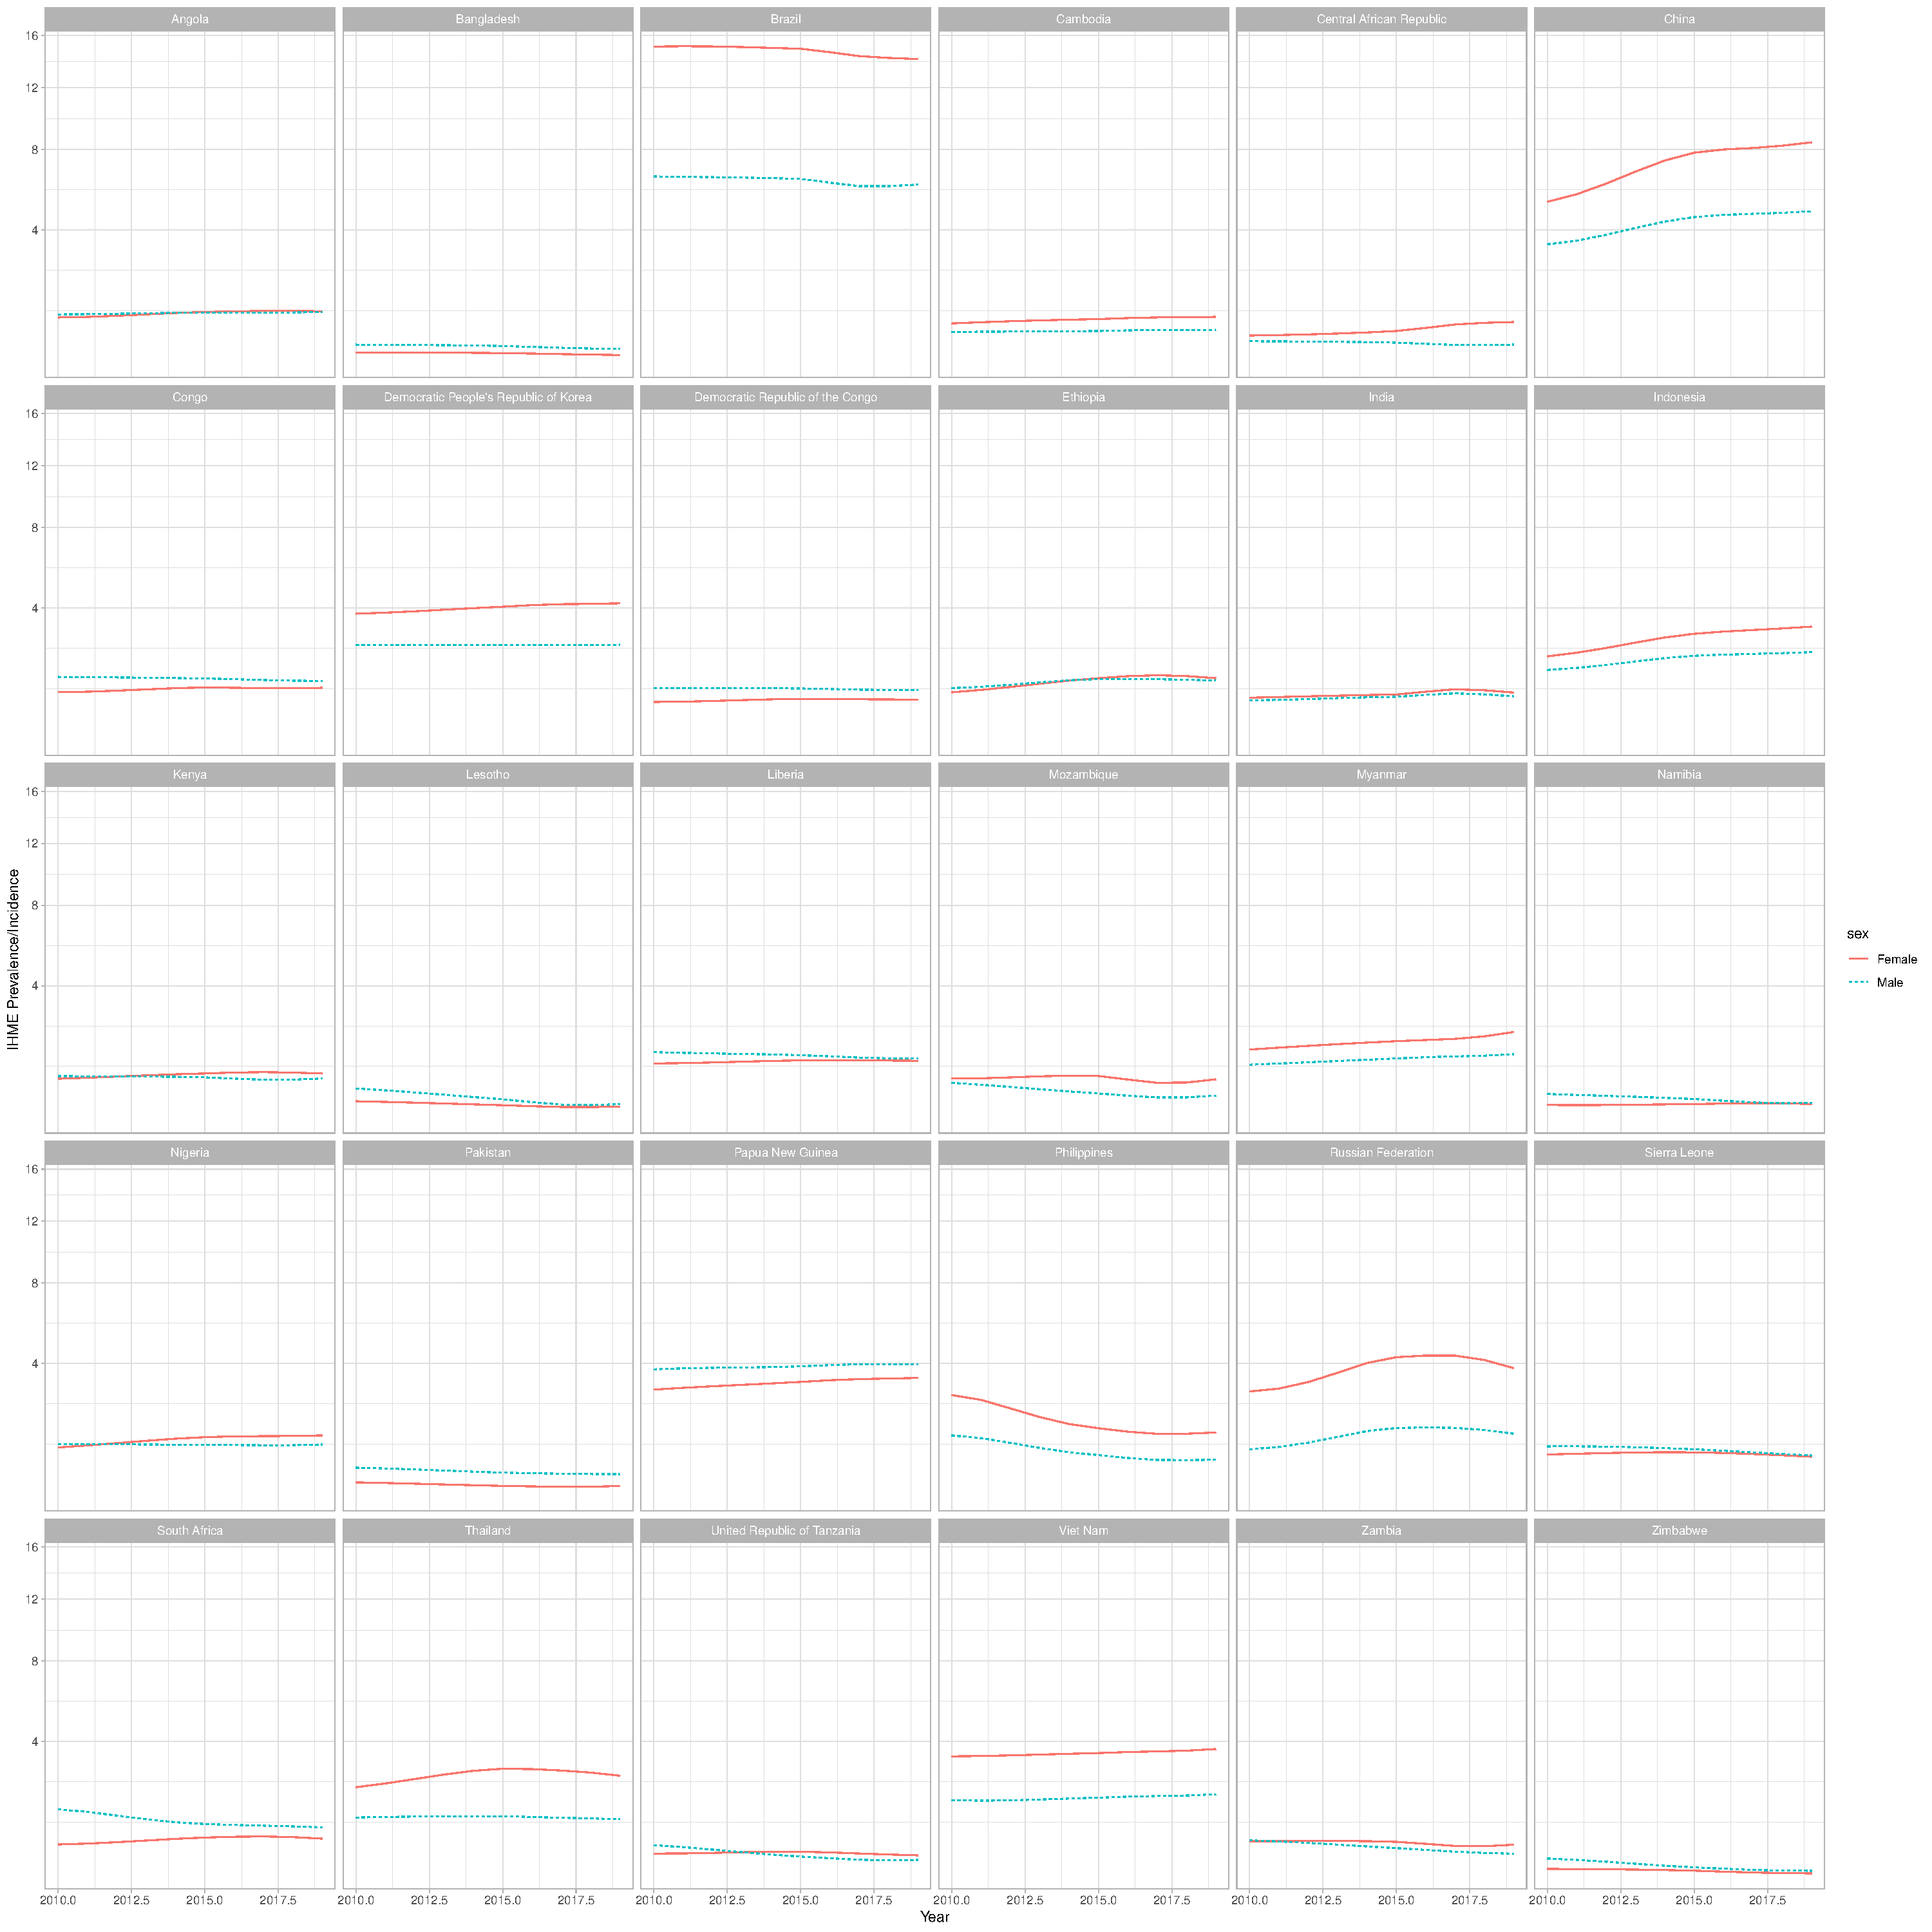
\includegraphics[width=1\textwidth]{../plots/aF6.pdf}
\caption{Implied duration over time}
\end{figure}

\FloatBarrier


\begin{figure}
\centering
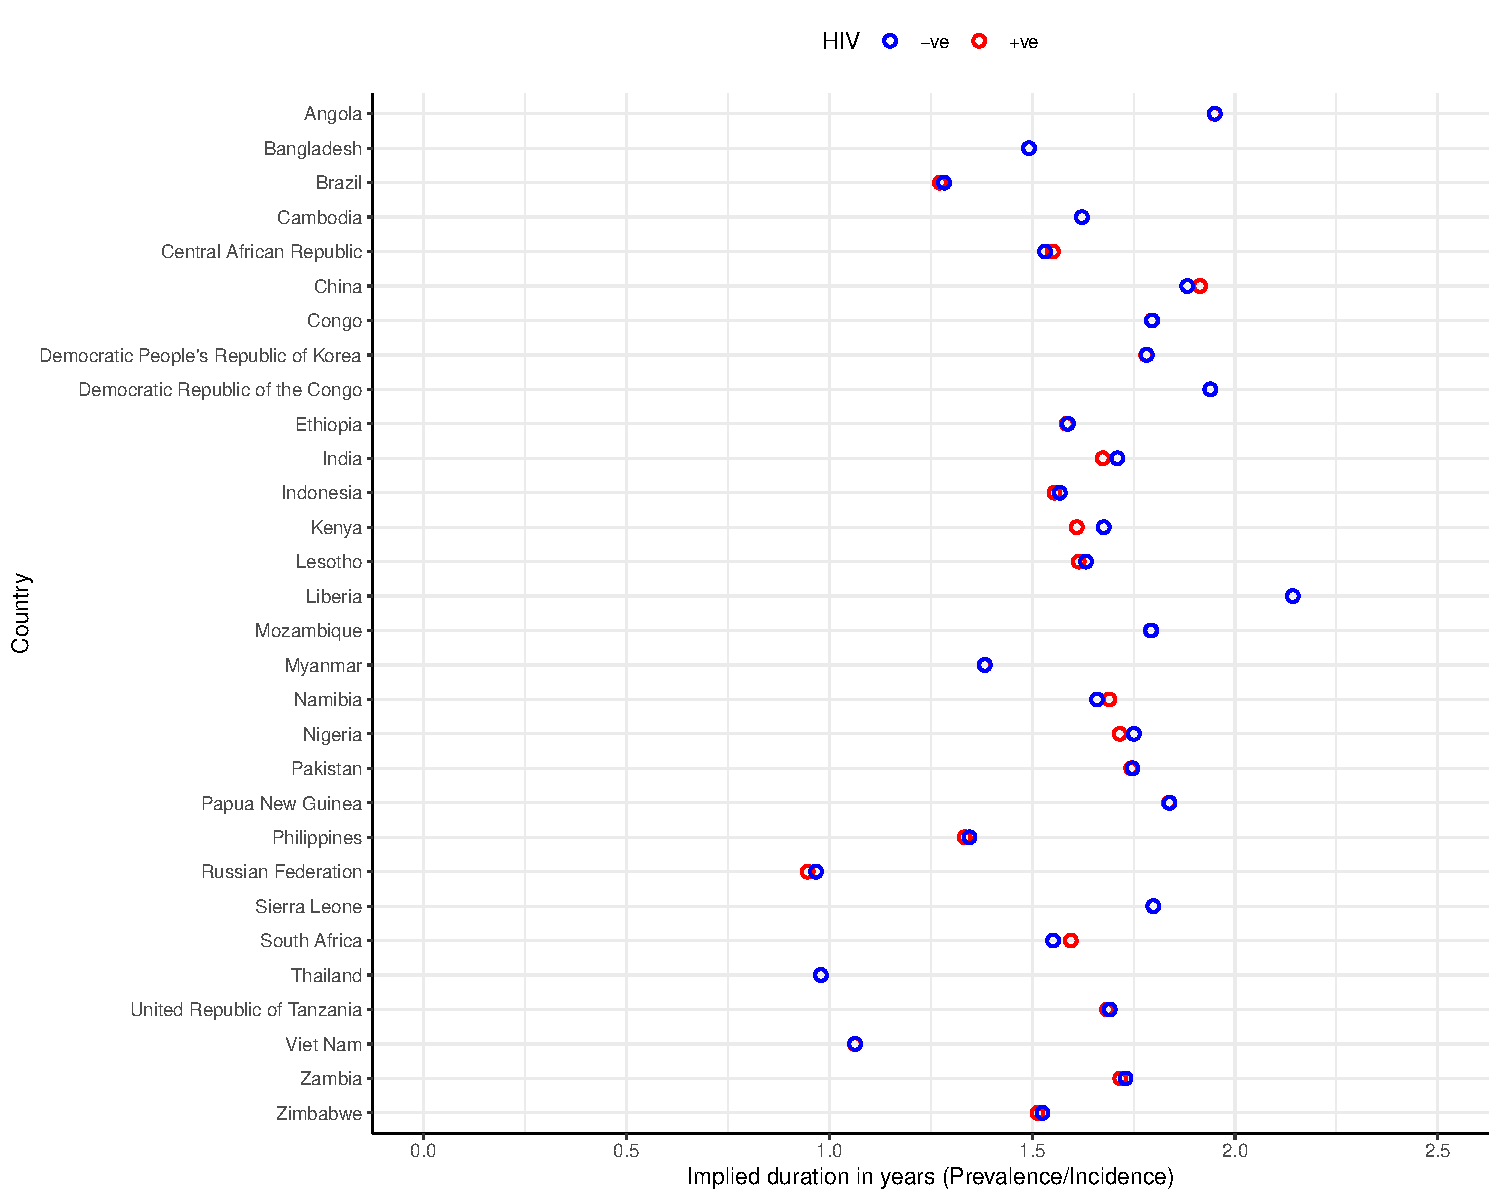
\includegraphics[width=1\textwidth]{../plots/aF7.pdf}
\caption{Implied duration by HIV status}
\end{figure}

\FloatBarrier


\begin{figure}
\centering
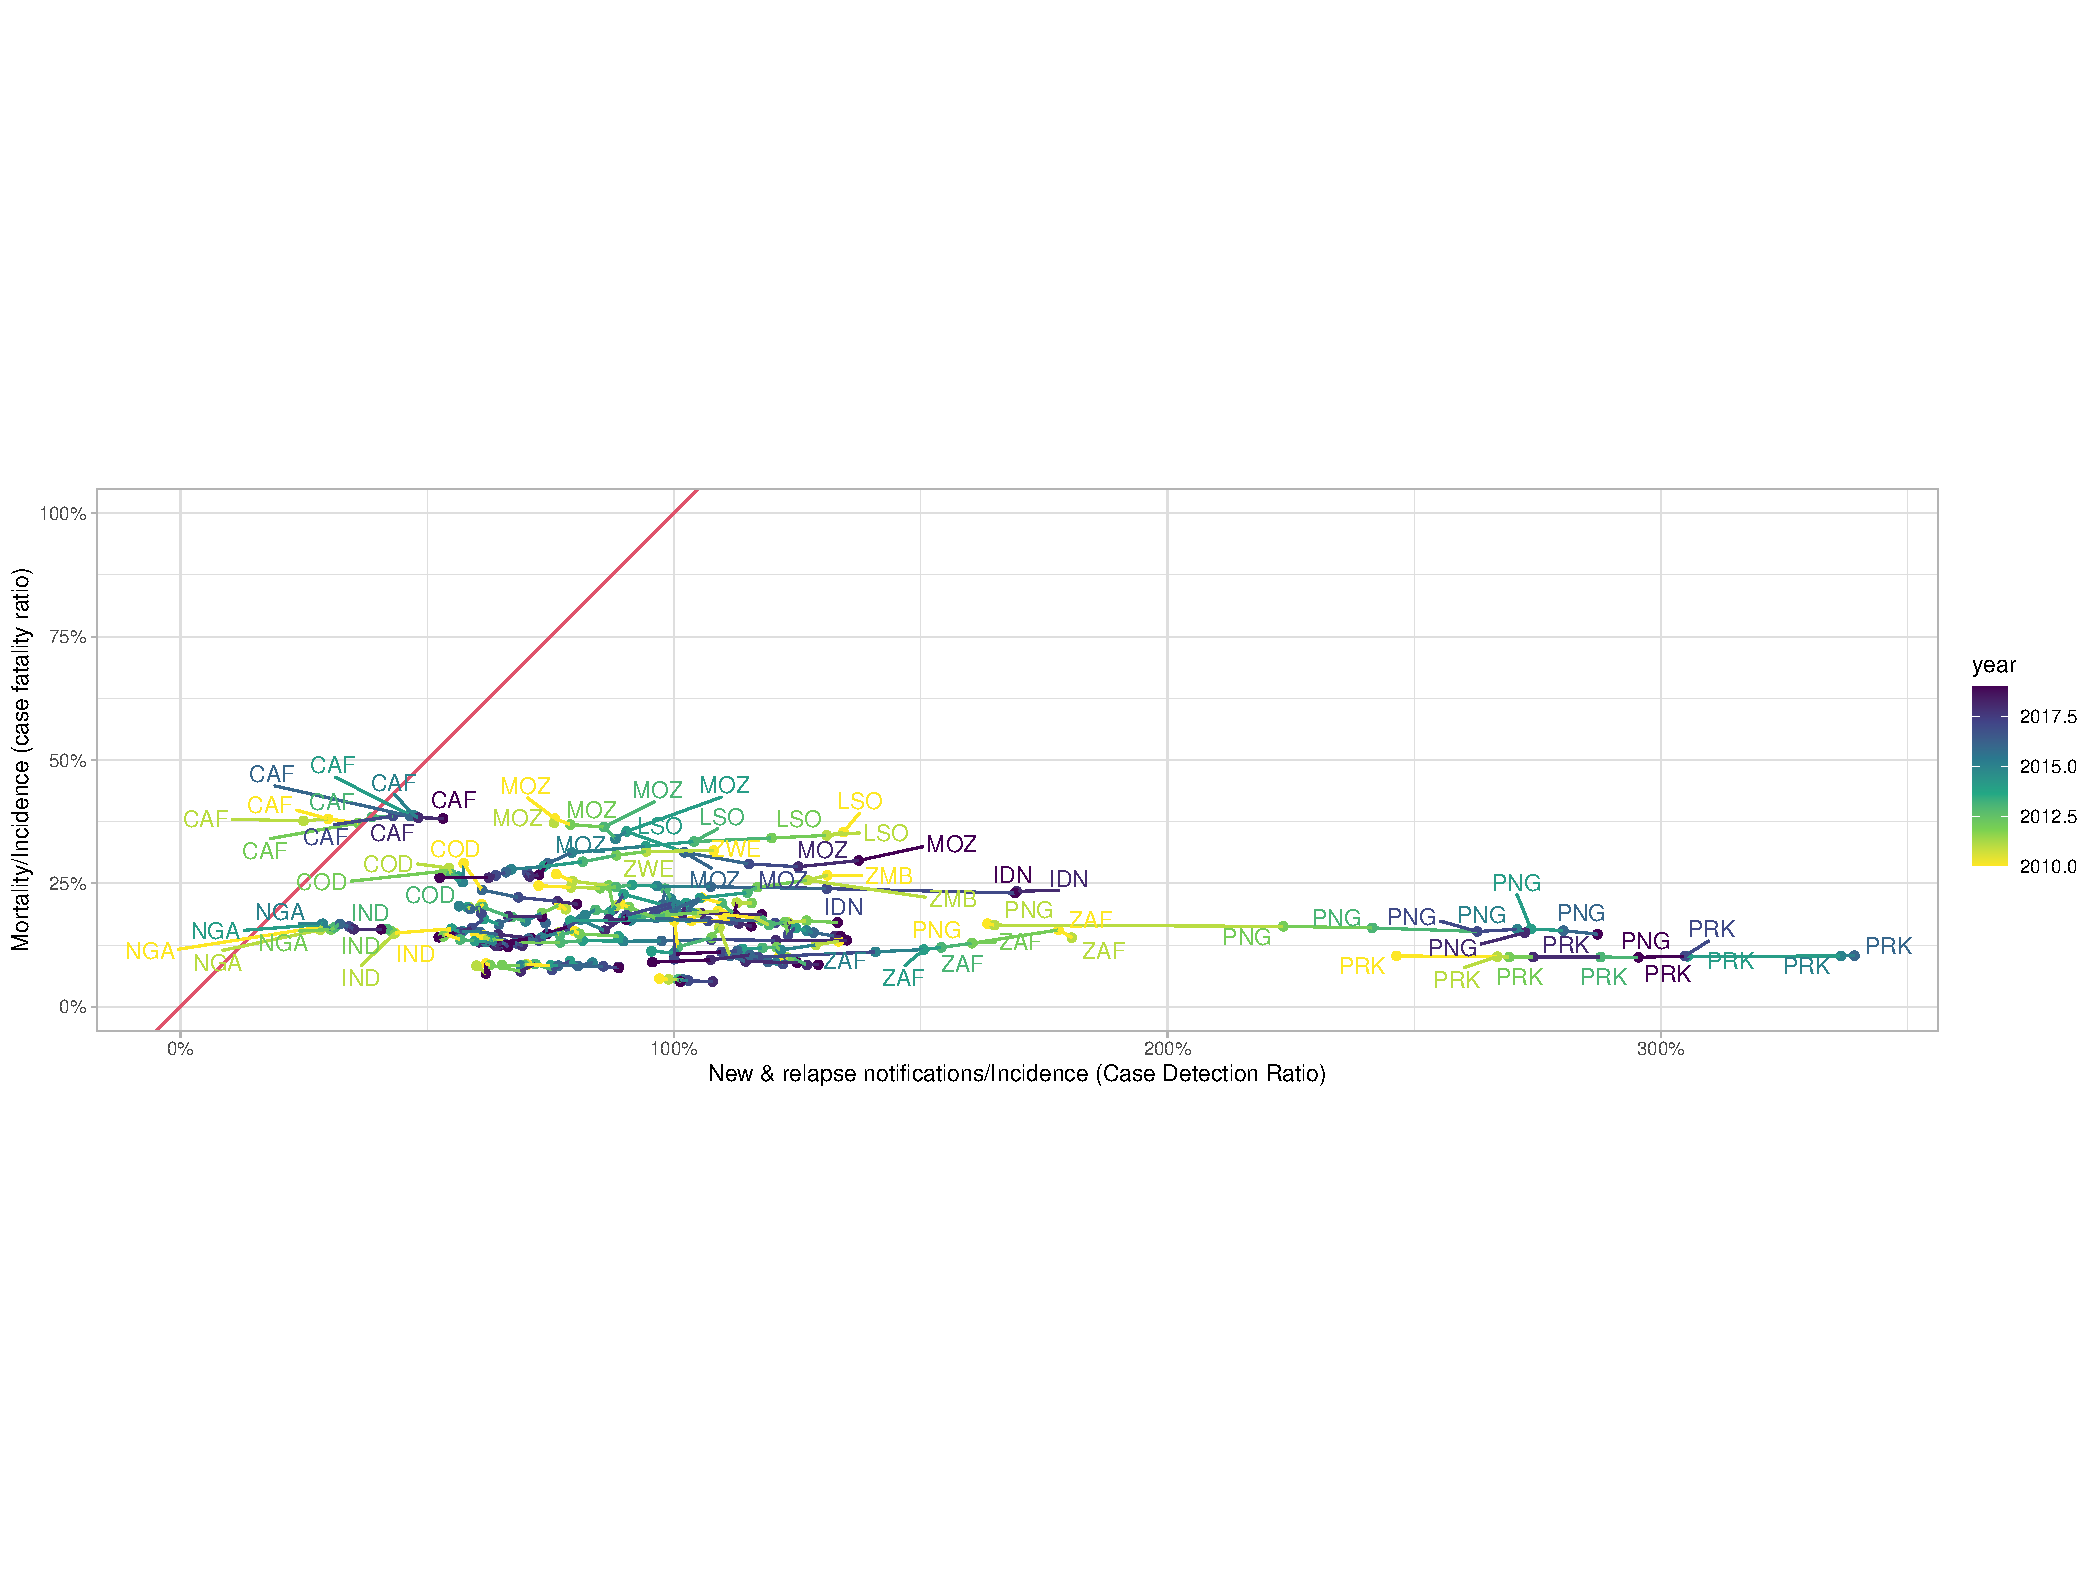
\includegraphics[width=0.8\textwidth]{../plots/aF8.pdf}
\caption{Case Fatality Ratio vs Case Detection Ratio}
\end{figure}
\end{document}